%%%%%%%%%%%%%%%%%%%%%%%%%%%%%%%%%%%%%%%%%%%%%%%%%%%%%%%%%%%%%%%%%%%%%%%%%%%%%%%%
%2345678901234567890123456789012345678901234567890123456789012345678901234567890
%        1         2         3         4         5         6         7         8

\documentclass[letterpaper, 10 pt, conference]{ieeeconf}  % Comment this line out
                                                          % if you need a4paper
%\documentclass[a4paper, 10pt, conference]{ieeeconf}      % Use this line for a4
                                                          % paper

\IEEEoverridecommandlockouts                              % This command is only
                                                          % needed if you want to
                                                          % use the \thanks command
\overrideIEEEmargins
% See the \addtolength command later in the file to balance the column lengths
% on the last page of the document

\usepackage[utf8]{inputenc}
\usepackage[T1]{fontenc}

% The following packages can be found on http:\\www.ctan.org
\usepackage{graphicx} % for pdf, bitmapped graphics files
%\usepackage{epsfig} % for postscript graphics files
%\usepackage{mathptmx} % assumes new font selection scheme installed
%\usepackage{mathptmx} % assumes new font selection scheme installed
%\usepackage{amsmath} % assumes amsmath package installed
%\usepackage{amssymb}  % assumes amsmath package installed

% configure your listings style
\usepackage{listings}
\lstset{
	tabsize=3,
	extendedchars=true,
	frame=single,
	showstringspaces=true,
	%numbers=left,
	numberstyle=\small,
	breakautoindent=true
}


\title{\LARGE \bf
Technical Report : OPCUA-Netzwerk
}

\author{Johannes Horst, Manuel Zimmermann, Patrick Sabau, Saniye Ogul, Stefan Ries und Tobias Schotter}% <-this % stops a space



\begin{document}

\maketitle
\thispagestyle{empty}
\pagestyle{empty}


%input erzeugt keine neue Seite, include schon
%zum schreiben ist es mit include übersichtlicher, aber das finale PDF sollte mit input erzeugt werden

\section{EINLEITUNG}\label{ch:einleitung}

Ziel dieses Projektes soll die Entwicklung eines Sensor-Netzwerks für den Heimbereich auf Basis von OPC-UA sein. 
Verschiedene Sensorknoten sollen mit entsprechender Sensorik und Aktorik ausgestattet sein, um bestimmte Daten des eigenen Zuhauses zu sammeln. 
Eine grafische Oberfläche ermöglicht dem Nutzer das Abrufen der Daten und außerdem Steuerungsfunktionalitäten, um z.B. eine Heizung oder eine Lüftungsanlage ein- bzw. auszuschalten. 
Hierdurch ergeben sich große Energiesparpotentiale, da man so nur lüftet bzw. heizt, wenn die Luftqualität/Temperatur dies erfordert.  

OPC-UA steht hierbei für „Open Platform Communication – Unified Architecture“ und ist eine aktuelle Technologie aus dem Industrie-4.0-Umfeld. OPC-UA soll die plattformunabhängige Machine-to-Machine Kommunikation ermöglichen. 
Dies wird durch ein zu modellierendes Informationsmodell möglich, welches den realen Sachverhalt abbildet und von einem zentralen Server verwaltet wird. 
Clients können sich mit dem Server verbinden und dort relevante Informationen ablegen bzw. diese abrufen oder durch Publish/Subscribe auch vom Server Daten erhalten. Die Informationen werden auf dem Server hierbei in einer Baumstruktur verwaltet. 
Durch die entsprechende Modellierung der Knoten des Baums erhalten diese z.B. durch die Festlegung eigener Datentypen eine semantische Bedeutung.

\section{Sensoren/Aktoren und Kommunikation}\label{ch:sensoren_kommunikation}

\newline Die verwendete Hardware-Plattform ist bei allen Sensorknoten ein Raspberry-Pi. Da der vorliegende Anwendungsfall keine große Leistungsfähigkeit der Hardware benötigt, wird für die Sensorknoten ein Model 3B verwendet. Um skalierbar zu bleiben und auch einen Puffer an Leistung für eventuelle zukünftige Funktionalitäten zu haben, wird für den Server ein Raspberry-Pi Model 4 verwendet.
\newline Für das Auslesen der Sensoren und das Ansteuern der Aktoren werden zum einen direkt die GPIO-Pins des Raspberry-Pis verwendet und zum anderen dessen vorhandene I2C-Schnittstelle. Analoge Sensoren können vom Raspberry-Pi nicht direkt ausgelesen werden, da dieser über keine integrierten Analog-Digital-Converter (ADC) verfügt. Hierfür werden die im auf der Platine aufgebrachten Microcontroller vorhandenen ADCs verwendet. Deren Werte können ebenfalls über I2C abgefragt werden.
\newline Die gemessenen Werte werden je nach Art des Sensors entweder zyklisch abgefragt und mittels OPC-UA an den Server übergeben oder bei Werteänderung azyklisch per OPC-UA übertragen.

\subsection{OPC-UA Server}
Die Client Anwendung wurde ebenfalls in Python mit der gleichen Bibliothek verwirklicht. Außerdem wird hier neben dem Ansteuern/Auslesen der Sensoren/Aktoren auch die Kommunikation mit dem OPC-UA Server und eine Steuerungsfunktionalität direkt am Knoten mit den vorhandenen Buttons realisiert. 

\subsection{OPC-UA Clients}
\newline Die Client Anwendung wurde ebenfalls in Python mit der gleichen Bibliothek verwirklicht. Außerdem wird hier neben dem Ansteuern/Auslesen der Sensoren/Aktoren auch die Kommunikation mit dem OPC-UA Server und eine Steuerungsfunktionalität direkt am Knoten mit den vorhandenen Buttons realisiert. 
\newline Im Hauptskript \textbf{Client.py} werden zunächst alle Sensor- und Aktorobjekte angelegt, sowie benötigte Threads gestartet und Callbacks hinterlegt. 
\newline Im \textbf{„measurement\textunderscore thread“} werden Temperatur, Luftfeuchtigkeit, Luftdruck und Luftqualität einmal pro Minute abgefragt und die entsprechenden Werte auf dem Display aktualisiert, sowie an den OPC-UA Server übermittelt. Entsprechend des Wertes für Luftqualität werden die vorhandenen LEDs geschalten, bzw. zusätzlich über den vorhandenen Buzzer ein Alarmton ausgegeben.

\begin{table}[]
\centering
\begin{tabular}{|l|l|l|ll}
\cline{1-3}
\textbf{CO2-Gehalt}                        & \textbf{LED aktiv} & \textbf{Alarm} &  &  \\ \cline{1-3}
\textless 800 ppm                          & Grün               & -              &  &  \\ \cline{1-3}
\textgreater 800 ppm \& \textless 1200 ppm & Gelb               & -              &  &  \\ \cline{1-3}
\textgreater 1200 ppm                      & Rot                & +              &  &  \\ \cline{1-3}
\end{tabular}
\end{table}

\newline Der \textbf{Bewegungssensor} stellt einen Event-Handler zur Verfügung, der abonniert werden kann. Bei Auftreten einer Bewegung wird das Event ausgelöst und ruft die hinterlegte Callback-Funktion auf, welche dem OPC-UA Server Anwesenheit signalisiert. Sobald eine Minute lang keine Bewegung mehr gemessen wird, wird das Event erneut ausgelöst und die Callback-Funktion setzt den entsprechenden Wert im Informationsmodell auf Abwesenheit.
\newline Um auf dem \textbf{LCD-Display} unterschiedliche Texte (Screens) anzeigen zu können und außerdem eine Referenzmessung des Luftqualitätssensors auszulösen, wurde ebenfalls eine \textbf{Steuerungsfunktionalität} mittels der Buttons implementiert. Das LCD-Display führt intern eine Liste mit anzuzeigenden Texten, die durch Knopfdruck durchgeschalten werden können. Ebenfalls durch Knopfdruck kann die erwähnte Referenzmessung des Luftqualitätssensors eingestellt und gestartet werden.
\newline Für das Ansteuern des \textbf{LCD-Displays} aus OPC-UA heraus wurde hierfür ein eigener Screen hinterlegt. Bei Änderung des entsprechenden Wertes im Informationsmodell wird mittels \textbf{Publish/Subscribe} der anzuzeigende Text aktualisiert.

\section{BACKEND + DATENBANK}\label{ch:backend}

Das Backend wurde mit dem Framework \textbf{FastAPI} in Python umgesetzt und ist die einzige Schnittstelle zur Datenbank \textbf{MongoDB}.

\subsection{Datenbank}
Um eine MongoDB lokal (für die Entwicklung) zu starten:
\begin{itemize}
\item Herunterladen von MongoDB über die offizielle Website oder einen Package Manager (z.B. ABT)
\item Ausführung der in der ReadMe-Datei hinterlegten Konsolenbefehle
\end{itemize}
Die Datenbank wird dabei in der Standardkonfiguration genutzt, somit ist es nicht erforderlich Nutzer oder anderes anzulegen.
Lediglich sollte die Datenbank über den Standardport 27017 erreichbar sein.

MongoDB enthält zu Beginn einige Tabellen die zur Konfiguration und zur internen Konsistenz genutzt werden.
Die eigentlichen Daten werden dabei in einer neuen Datenbank (der Name dieser kann konfiguriert werden) gespeichert.
Eine solche Datenbank kann mehrere Collectionen beinhalten, das Äquivalent zu Tabellen in einer SQL Datenbank.
Diese Collectionen beinhalten i.d.R ähnliche Documente im Format BSON (Binary JSON). 

\subsection{Datenformat}
Es werden Datenformate genutzt, die jeweils in Collections gespeichert werden : \textbf{Sensoren}.

Listing \ref{lst:sensor_dtype} zeigt ein Sensor Objekt, wie es in der Datenbank gespeichert sein könnte.
\begin{lstlisting}[caption={Sensor Objekt},captionpos=b,showstringspaces=false, basicstyle=\small,label={lst:sensor_dtype}]
{
    "_id": ObjectID(abc123def456),
    "sensornode": "SensorNode_1",
    "sensorname": "BME280",
    "sensortyp" : "AirPressure",
    "unit"      : "hPa,
    "value"     : 1040.6999999999991,
    "timestamp" : "2022-12-06T15:15:28.112Z"
}
\end{lstlisting}

Das Feld \textbf{'\_id'} ist ein Primärschlüssel, welcher einzigartig ist und automatisch von MongoDB vergeben wird. 
Mit diesem können Objekte eindeutig referenziert werden.
Über \textbf{'sensornode'} wird die Bezeichnung der Nodes gespeichert.
Das Feld \textbf{'sensorname'} speichert den technischen Namen eines Sensors als String und das Feld \textbf{'sensortyp'} die tatsächliche Sensorbezeichnung. 
Durch Kombination dieser drei Werte können die Sensoren eindeutig zugeordnet, sowie im Frontend passend der per Name angezeigt werden.

Die Datenbankobjekte werden im Code als Pydantic Dataclasses hinterlegt, was das Parsen dieser Objekte (z.B. als JSON Payload) erleichtert. 
Dabei werden die Klassen mit dem Decorator \textbf{@dataclass} verziert und erhalten \textbf{TypeHints} mit entsprechden Datentypen

\begin{lstlisting}[language=python,caption={Sensor Dataclass},captionpos=b,showstringspaces=false, basicstyle=\small]
@dataclass
class Sensor_value_dto():
    sensornode: str
    sensorname: str
    sensortyp: str
    value: Union[float,bool]
    timestamp: datetime.datetime
    unit: str = ""
\end{lstlisting}

\begin{lstlisting}[language=python,caption={Actuator Dataclass},captionpos=b,showstringspaces=false, basicstyle=\small]
@dataclass
class actuator_list_dto:
    actuator_node : str
    actuator_act  : str
    actuator_value: Union[str,float,bool,None]
    actuator_dtype: str
\end{lstlisting}

\subsection{Backend}
Mittels dem Python Framework \textbf{FastAPI} werden diverse Endpoints bereitgestellt, die das Erstellen und Ausgeben der Datenobjekte ermöglichen.

Die Sensoren können über folgende Routen ausgegeben werden:
\begin{itemize}
\item \textbf{GET /sensornames}: Gibt eine Liste aller zur Verfügung stehenden Sensoren zurück.
\item \textbf{GET /sensornodes}: Gibt eine Liste aller zur Verfügung stehenden Knoten zurück.
\item \textbf{GET /sensorvalues/current}: Gibt den aktuellen Wert jedes Sensors zurück.
\item \textbf{GET /sensorvalues}: Gibt eine Liste von Sensoren zurück, welche sich nach ihren Attributen filtern lassen.
\end{itemize}

Die Aktoren können über folgende Routen ausgelesen und gesteuert werden:
\begin{itemize}
\item \textbf{GET /actuatornames}: Gibt eine Liste aller zur Verfügung stehenden Aktorenbezeichnungen zurück.
\item \textbf{GET /actuators}: Gibt eine Liste von JSON-Objekten zurück mit entsprechenden Informationen einzelner Aktoren.
\item \textbf{GET /actuators/filter\_by\_actuatorname}: Gibt eine Liste von JSON-Objekten, gefiltert bei Aktorbezeichnung zurück.
\item \textbf{PUT /actuators}: Ermöglicht per Übergabe von Aktorenknoten und Bezeichnung den Wert des Aktors zu ändern.
\end{itemize}

Die Endpunkte nutzen dabei ein automatisiertes Umwandeln zu entsprechenden Dataclasses.
Dies sorgt dafür, dass Pflichtfelder übergeben und nicht benötigte Elemente verworfen werden.
Über einen PyMongo Client werden diese Dataclasses also entweder von der Clientanfrage zur Datenbank weitergeleitet, oder umgekehrt aus der Datenbank zum Client.
Die Verbindung erfolgt dabei über eine \textbf{MONGO\_URI}, welche Hostnamen und Port beinhaltet. Dieser String sieht wie folgt aus: \textit{mongodb://localhost:27017/}. \\
Als tatsächlicher Webserver wird \textbf{uvicorn} genutzt, welcher im \textbf{\_\_main\_\_.py} gestartet wird. Dies ermöglicht es, das Backend mittels des Befehlt \textit{python -m backend} zu starten.

%\subsection{Tests}
%In einem separaten Testscript \textbf{test\_backend.py} werden die Routen getestet. 
%Hierbei wird jedoch eine Testtabelle in der Datenbank genutzt, um nicht mit anderen Daten zu interferieren. 
%In einer Setup-Methode werden dabei die Referenzen auf die Tabelle ausgetauscht. 
%Der Server wird ebenfalls durch einen \textbf{TestClient} ersetzt, welcher in dem FastAPI Framework integriert ist.
%Die Tests können mittels des Befehls \textit{python -m pytest -s} gestartet werden.

\section{FRONTEND}\label{ch:frontend}

Das Frontend wurde mithilfe des Admin-Dashboard ngx-admin auf Basis von Angular 9+ und Nebular entwickelt. Mittels Angular wird eine Weboberfläche komponentenbasiert zur Verfügung gestellt. Für die serverseitige Anwendung benötigt Angular zudem Node.js, eine JavaScript-Laufzeitumgebung. Zudem wird ngx-admin mit dem Eva Design System unterstützt, um UI-Design zu vereinfachen. 

\subsection{Architektur}

In der unteren Abbildung \ref{fig:frontend} ist die Architektur des Frontends zu sehen. Eine Komponente besteht aus einem Template (HTML-Datei) und einem Style (SCSS-Datei). Diese werden als Metadaten im Dekorator der Komponente festgelegt und stellen die Ansicht dar. Mithilfe der Datenbindung kann das Template mit der Komponente Daten austauschen und gegebenenfalls Events ausführen. Bei Bedarf können Komponenten durch die Dependency Injection Zugriff auf eine Serviceklasse erhalten. Somit können wiederverwendbare Funktionen oder Daten aus dem Backend zur Verfügung gestellt werden. In den Modulen werden Komponenten, Module, Services usw. gruppiert und verwaltet. In Angular werden zwei Modularten unterschieden. Jedes Angular Projekt besitzt ein Root-Modul, das app.module.ts heißt. Diese ist dazu da, um die gesamte Webanwendung zu verwalten und diese wird beim Start der Anwendung als erstes geladen und initialisiert. Mit Feature-Modulen kann der Code, der sich auf eine bestimmte Funktionalität oder ein bestimmtes Feature bezieht, von anderem Code getrennt werden und bleibt somit organisiert.
Das Frontend wird auf dem Raspberry Pi Server gehostet. Für das Hosting wird ein Apache 2 Webserver verwendet.
\begin{figure}[thpb]
      \centering
      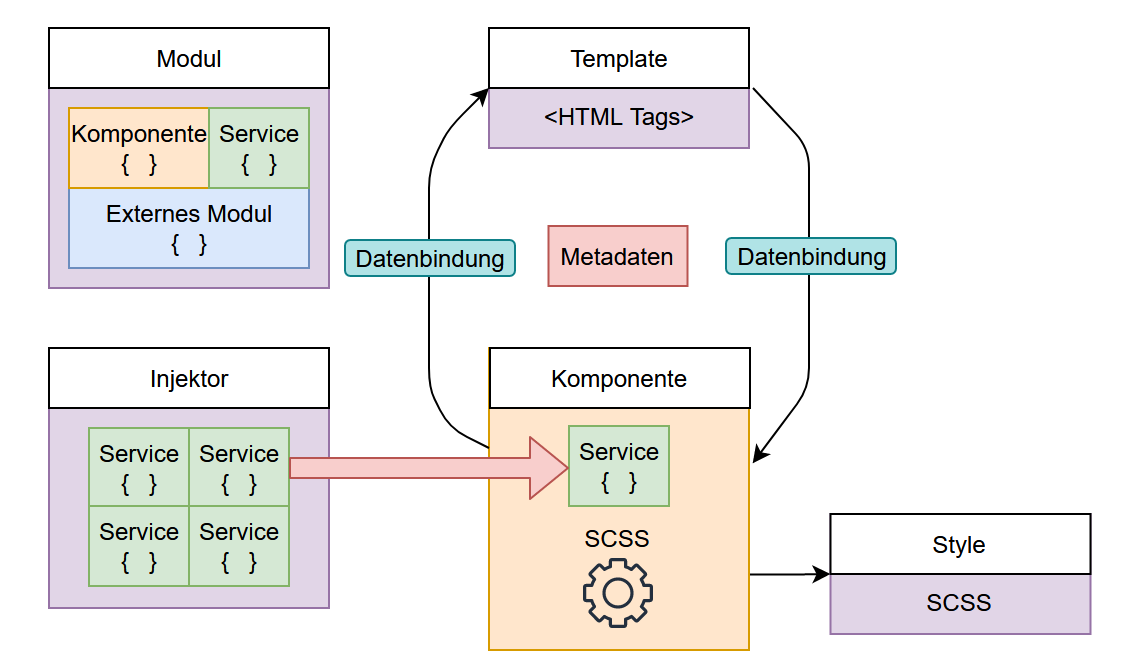
\includegraphics[scale=0.55]{abbildungen/frontend_architecture.PNG}
      \caption{Angular Architektur des Projektes}
      \label{fig:frontend}
 \end{figure}


\subsection{Entwickelte Komponenten}
Für alle Diagramme wurde die Bibliothek ECharts verwendet.
Zusätzlich zu den vorhandenen Komponenten vom ngx-admin wurden folgende weitere Komponenten entwickelt.

\begin{itemize}
 \item \textbf{AirQualityChart} Bildet die Werte des Luftqualitätssensors in einem Liniendiagramm ab.
 \item \textbf{AirQuality} Visualisiert die Werte des Luftqualitätssensors unter Verwendung der AirQualityChart Komponente.
 \item \textbf{buzzer-frequenzy}	Ein Eingabefeld zum Festsetzen der Frequenz des Piezoelements.
 \item \textbf{gant} Das Gantt-Diagramm zeigt an, von wann bis wann der Bewegungsmelder Anwesenheit, bzw. Abwesenheit erkannt hat. 
 \item \textbf{lcd-input} Ein Eingabefeld zum Festsetzen des LCD-Displays auf dem Sensorknoten.
 \item \textbf{lineChartComponent} Ein universell verwendbares Liniendiagramm.
 \item \textbf{switch} Ein Knopf, der an- und ausgeschaltet werden kann.
 \item \textbf{temperatureGauge} Ein Tachometer zum Visualisieren von verschiedenen Werten.
 \item \textbf{tempSensorCard} Kombination aus dem LineChartComponent und dem temperatureGauge Komponente. Stellt eine zweiseitige Karte dar, die auf der einen Seite Luftdruck, Luftfeuchtigkeit und Temperatur in einem Liniendiagramm darstellt und auf der anderen Seite ein Tachometer mit den aktuellen Werten.
 \item \textbf{sensornode-dashbord} Stellt das eigentliche Dasboard für jeden Knoten dar. In dieser Komponente werden die oben genannten Komponenten des jeweiligen Sensorknotens dargestellt. Jede Komponente wird als einzelne Karte dargestellt. Diese können sich je nach Bildschirmgröße passend anordnen.
 \item \textbf{led-display} Zeigt die LED-Anzeige des aktuellen Knotens.
 \item \textbf{Header (modifiziert)} Der vorhandene Header wurde modifiziert, um eine Zeitspanne auswählen zu können.
\end{itemize}

\subsection{Entwickelte Services}

\begin{itemize}
 \item \textbf{BackendDataService} Ist für die Kommunikation mit dem Backend zuständig. Zum Abfragen und Senden von Daten.
 \item \textbf{DashboardFunctionalityService} Auslagerung der Funktionen für die sensornode-dashboard Komponente.
 \item \textbf{SharedDataService} Stellt allen Komponenten ein Observable des ausgewählten Zeitraums und der aktuellen Sensorknoten-ID zur Verfügung.
\end{itemize}
\subsection{Routing}
Alle verfügbaren Seiten im Projekt repräsentieren ein Dashboard eines Sensorknotens.
Zugänglich sind diese über die URL: /pages/{Knoten-ID}. Siehe Listing 5.
\begin{lstlisting}[caption={Knoten-ID Routing},captionpos=b,showstringspaces=false, basicstyle=\small]
    {
      path: ':id',
      component: SensorNodeDashboardComponent
    }
\end{lstlisting}
Alle verfügbaren Knoten werden am Anfang aus dem Backend abgerufen, und anschließend links im Navigator als Menüpunkt angezeigt. Auf dem Dashboard des einzelnen Knotens werden über die aktuelle Knoten-ID die Anfragen an das Backend gesendet.
\section{AUSBLICK}\label{ch:ausblick}

%\section{EINLEITUNG}\label{ch:einleitung}

Ziel dieses Projektes soll die Entwicklung eines Sensor-Netzwerks für den Heimbereich auf Basis von OPC-UA sein. 
Verschiedene Sensorknoten sollen mit entsprechender Sensorik und Aktorik ausgestattet sein, um bestimmte Daten des eigenen Zuhauses zu sammeln. 
Eine grafische Oberfläche ermöglicht dem Nutzer das Abrufen der Daten und außerdem Steuerungsfunktionalitäten, um z.B. eine Heizung oder eine Lüftungsanlage ein- bzw. auszuschalten. 
Hierdurch ergeben sich große Energiesparpotentiale, da man so nur lüftet bzw. heizt, wenn die Luftqualität/Temperatur dies erfordert.  

OPC-UA steht hierbei für „Open Platform Communication – Unified Architecture“ und ist eine aktuelle Technologie aus dem Industrie-4.0-Umfeld. OPC-UA soll die plattformunabhängige Machine-to-Machine Kommunikation ermöglichen. 
Dies wird durch ein zu modellierendes Informationsmodell möglich, welches den realen Sachverhalt abbildet und von einem zentralen Server verwaltet wird. 
Clients können sich mit dem Server verbinden und dort relevante Informationen ablegen bzw. diese abrufen oder durch Publish/Subscribe auch vom Server Daten erhalten. Die Informationen werden auf dem Server hierbei in einer Baumstruktur verwaltet. 
Durch die entsprechende Modellierung der Knoten des Baums erhalten diese z.B. durch die Festlegung eigener Datentypen eine semantische Bedeutung.

%\section{BACKEND + DATENBANK}\label{ch:backend}

Das Backend wurde mit dem Framework \textbf{FastAPI} in Python umgesetzt und ist die einzige Schnittstelle zur Datenbank \textbf{MongoDB}.

\subsection{Datenbank}
Um eine MongoDB lokal (für die Entwicklung) zu starten:
\begin{itemize}
\item Herunterladen von MongoDB über die offizielle Website oder einen Package Manager (z.B. ABT)
\item Ausführung der in der ReadMe-Datei hinterlegten Konsolenbefehle
\end{itemize}
Die Datenbank wird dabei in der Standardkonfiguration genutzt, somit ist es nicht erforderlich Nutzer oder anderes anzulegen.
Lediglich sollte die Datenbank über den Standardport 27017 erreichbar sein.

MongoDB enthält zu Beginn einige Tabellen die zur Konfiguration und zur internen Konsistenz genutzt werden.
Die eigentlichen Daten werden dabei in einer neuen Datenbank (der Name dieser kann konfiguriert werden) gespeichert.
Eine solche Datenbank kann mehrere Collectionen beinhalten, das Äquivalent zu Tabellen in einer SQL Datenbank.
Diese Collectionen beinhalten i.d.R ähnliche Documente im Format BSON (Binary JSON). 

\subsection{Datenformat}
Es werden Datenformate genutzt, die jeweils in Collections gespeichert werden : \textbf{Sensoren}.

Listing \ref{lst:sensor_dtype} zeigt ein Sensor Objekt, wie es in der Datenbank gespeichert sein könnte.
\begin{lstlisting}[caption={Sensor Objekt},captionpos=b,showstringspaces=false, basicstyle=\small,label={lst:sensor_dtype}]
{
    "_id": ObjectID(abc123def456),
    "sensornode": "SensorNode_1",
    "sensorname": "BME280",
    "sensortyp" : "AirPressure",
    "unit"      : "hPa,
    "value"     : 1040.6999999999991,
    "timestamp" : "2022-12-06T15:15:28.112Z"
}
\end{lstlisting}

Das Feld \textbf{'\_id'} ist ein Primärschlüssel, welcher einzigartig ist und automatisch von MongoDB vergeben wird. 
Mit diesem können Objekte eindeutig referenziert werden.
Über \textbf{'sensornode'} wird die Bezeichnung der Nodes gespeichert.
Das Feld \textbf{'sensorname'} speichert den technischen Namen eines Sensors als String und das Feld \textbf{'sensortyp'} die tatsächliche Sensorbezeichnung. 
Durch Kombination dieser drei Werte können die Sensoren eindeutig zugeordnet, sowie im Frontend passend der per Name angezeigt werden.

Die Datenbankobjekte werden im Code als Pydantic Dataclasses hinterlegt, was das Parsen dieser Objekte (z.B. als JSON Payload) erleichtert. 
Dabei werden die Klassen mit dem Decorator \textbf{@dataclass} verziert und erhalten \textbf{TypeHints} mit entsprechden Datentypen

\begin{lstlisting}[language=python,caption={Sensor Dataclass},captionpos=b,showstringspaces=false, basicstyle=\small]
@dataclass
class Sensor_value_dto():
    sensornode: str
    sensorname: str
    sensortyp: str
    value: Union[float,bool]
    timestamp: datetime.datetime
    unit: str = ""
\end{lstlisting}

\begin{lstlisting}[language=python,caption={Actuator Dataclass},captionpos=b,showstringspaces=false, basicstyle=\small]
@dataclass
class actuator_list_dto:
    actuator_node : str
    actuator_act  : str
    actuator_value: Union[str,float,bool,None]
    actuator_dtype: str
\end{lstlisting}

\subsection{Backend}
Mittels dem Python Framework \textbf{FastAPI} werden diverse Endpoints bereitgestellt, die das Erstellen und Ausgeben der Datenobjekte ermöglichen.

Die Sensoren können über folgende Routen ausgegeben werden:
\begin{itemize}
\item \textbf{GET /sensornames}: Gibt eine Liste aller zur Verfügung stehenden Sensoren zurück.
\item \textbf{GET /sensornodes}: Gibt eine Liste aller zur Verfügung stehenden Knoten zurück.
\item \textbf{GET /sensorvalues/current}: Gibt den aktuellen Wert jedes Sensors zurück.
\item \textbf{GET /sensorvalues}: Gibt eine Liste von Sensoren zurück, welche sich nach ihren Attributen filtern lassen.
\end{itemize}

Die Aktoren können über folgende Routen ausgelesen und gesteuert werden:
\begin{itemize}
\item \textbf{GET /actuatornames}: Gibt eine Liste aller zur Verfügung stehenden Aktorenbezeichnungen zurück.
\item \textbf{GET /actuators}: Gibt eine Liste von JSON-Objekten zurück mit entsprechenden Informationen einzelner Aktoren.
\item \textbf{GET /actuators/filter\_by\_actuatorname}: Gibt eine Liste von JSON-Objekten, gefiltert bei Aktorbezeichnung zurück.
\item \textbf{PUT /actuators}: Ermöglicht per Übergabe von Aktorenknoten und Bezeichnung den Wert des Aktors zu ändern.
\end{itemize}

Die Endpunkte nutzen dabei ein automatisiertes Umwandeln zu entsprechenden Dataclasses.
Dies sorgt dafür, dass Pflichtfelder übergeben und nicht benötigte Elemente verworfen werden.
Über einen PyMongo Client werden diese Dataclasses also entweder von der Clientanfrage zur Datenbank weitergeleitet, oder umgekehrt aus der Datenbank zum Client.
Die Verbindung erfolgt dabei über eine \textbf{MONGO\_URI}, welche Hostnamen und Port beinhaltet. Dieser String sieht wie folgt aus: \textit{mongodb://localhost:27017/}. \\
Als tatsächlicher Webserver wird \textbf{uvicorn} genutzt, welcher im \textbf{\_\_main\_\_.py} gestartet wird. Dies ermöglicht es, das Backend mittels des Befehlt \textit{python -m backend} zu starten.

%\subsection{Tests}
%In einem separaten Testscript \textbf{test\_backend.py} werden die Routen getestet. 
%Hierbei wird jedoch eine Testtabelle in der Datenbank genutzt, um nicht mit anderen Daten zu interferieren. 
%In einer Setup-Methode werden dabei die Referenzen auf die Tabelle ausgetauscht. 
%Der Server wird ebenfalls durch einen \textbf{TestClient} ersetzt, welcher in dem FastAPI Framework integriert ist.
%Die Tests können mittels des Befehls \textit{python -m pytest -s} gestartet werden.

%\section{FRONTEND}\label{ch:frontend}

Das Frontend wurde mithilfe des Admin-Dashboard ngx-admin auf Basis von Angular 9+ und Nebular entwickelt. Mittels Angular wird eine Weboberfläche komponentenbasiert zur Verfügung gestellt. Für die serverseitige Anwendung benötigt Angular zudem Node.js, eine JavaScript-Laufzeitumgebung. Zudem wird ngx-admin mit dem Eva Design System unterstützt, um UI-Design zu vereinfachen. 

\subsection{Architektur}

In der unteren Abbildung \ref{fig:frontend} ist die Architektur des Frontends zu sehen. Eine Komponente besteht aus einem Template (HTML-Datei) und einem Style (SCSS-Datei). Diese werden als Metadaten im Dekorator der Komponente festgelegt und stellen die Ansicht dar. Mithilfe der Datenbindung kann das Template mit der Komponente Daten austauschen und gegebenenfalls Events ausführen. Bei Bedarf können Komponenten durch die Dependency Injection Zugriff auf eine Serviceklasse erhalten. Somit können wiederverwendbare Funktionen oder Daten aus dem Backend zur Verfügung gestellt werden. In den Modulen werden Komponenten, Module, Services usw. gruppiert und verwaltet. In Angular werden zwei Modularten unterschieden. Jedes Angular Projekt besitzt ein Root-Modul, das app.module.ts heißt. Diese ist dazu da, um die gesamte Webanwendung zu verwalten und diese wird beim Start der Anwendung als erstes geladen und initialisiert. Mit Feature-Modulen kann der Code, der sich auf eine bestimmte Funktionalität oder ein bestimmtes Feature bezieht, von anderem Code getrennt werden und bleibt somit organisiert.
Das Frontend wird auf dem Raspberry Pi Server gehostet. Für das Hosting wird ein Apache 2 Webserver verwendet.
\begin{figure}[thpb]
      \centering
      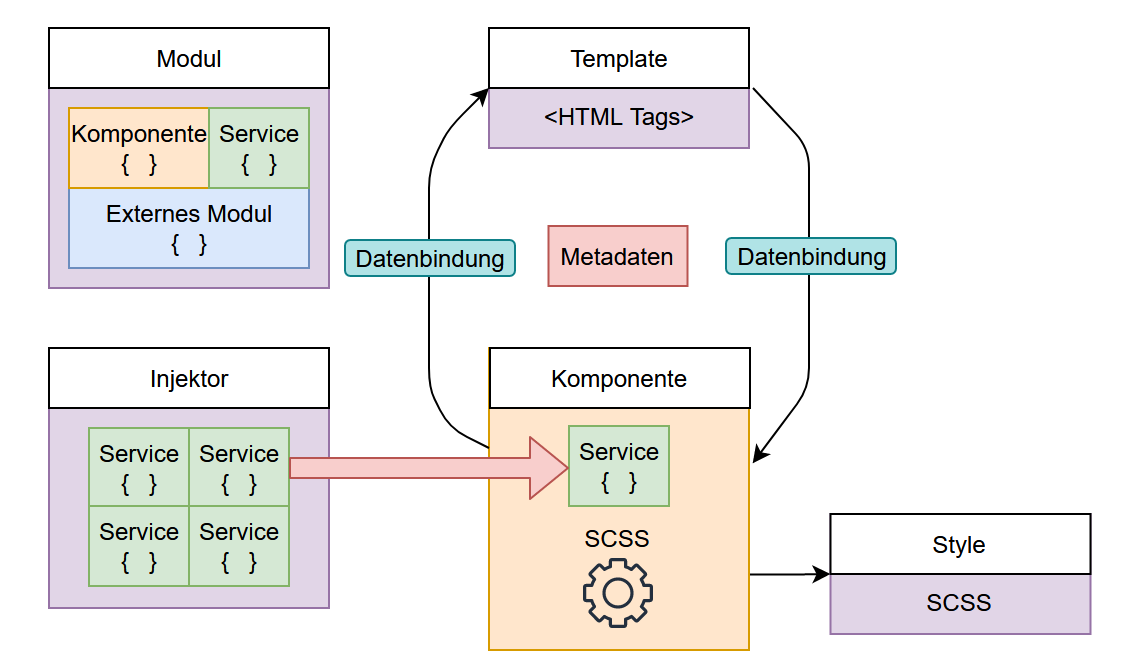
\includegraphics[scale=0.55]{abbildungen/frontend_architecture.PNG}
      \caption{Angular Architektur des Projektes}
      \label{fig:frontend}
 \end{figure}


\subsection{Entwickelte Komponenten}
Für alle Diagramme wurde die Bibliothek ECharts verwendet.
Zusätzlich zu den vorhandenen Komponenten vom ngx-admin wurden folgende weitere Komponenten entwickelt.

\begin{itemize}
 \item \textbf{AirQualityChart} Bildet die Werte des Luftqualitätssensors in einem Liniendiagramm ab.
 \item \textbf{AirQuality} Visualisiert die Werte des Luftqualitätssensors unter Verwendung der AirQualityChart Komponente.
 \item \textbf{buzzer-frequenzy}	Ein Eingabefeld zum Festsetzen der Frequenz des Piezoelements.
 \item \textbf{gant} Das Gantt-Diagramm zeigt an, von wann bis wann der Bewegungsmelder Anwesenheit, bzw. Abwesenheit erkannt hat. 
 \item \textbf{lcd-input} Ein Eingabefeld zum Festsetzen des LCD-Displays auf dem Sensorknoten.
 \item \textbf{lineChartComponent} Ein universell verwendbares Liniendiagramm.
 \item \textbf{switch} Ein Knopf, der an- und ausgeschaltet werden kann.
 \item \textbf{temperatureGauge} Ein Tachometer zum Visualisieren von verschiedenen Werten.
 \item \textbf{tempSensorCard} Kombination aus dem LineChartComponent und dem temperatureGauge Komponente. Stellt eine zweiseitige Karte dar, die auf der einen Seite Luftdruck, Luftfeuchtigkeit und Temperatur in einem Liniendiagramm darstellt und auf der anderen Seite ein Tachometer mit den aktuellen Werten.
 \item \textbf{sensornode-dashbord} Stellt das eigentliche Dasboard für jeden Knoten dar. In dieser Komponente werden die oben genannten Komponenten des jeweiligen Sensorknotens dargestellt. Jede Komponente wird als einzelne Karte dargestellt. Diese können sich je nach Bildschirmgröße passend anordnen.
 \item \textbf{led-display} Zeigt die LED-Anzeige des aktuellen Knotens.
 \item \textbf{Header (modifiziert)} Der vorhandene Header wurde modifiziert, um eine Zeitspanne auswählen zu können.
\end{itemize}

\subsection{Entwickelte Services}

\begin{itemize}
 \item \textbf{BackendDataService} Ist für die Kommunikation mit dem Backend zuständig. Zum Abfragen und Senden von Daten.
 \item \textbf{DashboardFunctionalityService} Auslagerung der Funktionen für die sensornode-dashboard Komponente.
 \item \textbf{SharedDataService} Stellt allen Komponenten ein Observable des ausgewählten Zeitraums und der aktuellen Sensorknoten-ID zur Verfügung.
\end{itemize}
\subsection{Routing}
Alle verfügbaren Seiten im Projekt repräsentieren ein Dashboard eines Sensorknotens.
Zugänglich sind diese über die URL: /pages/{Knoten-ID}. Siehe Listing 5.
\begin{lstlisting}[caption={Knoten-ID Routing},captionpos=b,showstringspaces=false, basicstyle=\small]
    {
      path: ':id',
      component: SensorNodeDashboardComponent
    }
\end{lstlisting}
Alle verfügbaren Knoten werden am Anfang aus dem Backend abgerufen, und anschließend links im Navigator als Menüpunkt angezeigt. Auf dem Dashboard des einzelnen Knotens werden über die aktuelle Knoten-ID die Anfragen an das Backend gesendet.
%\include{kapitel/sesoren}
%\section{AUSBLICK}\label{ch:ausblick}



%%%%%%%%%%%%%%%%%%%%%%%%%%%%%%%%%%%%%%%%%%%%%%%%%%%%%%%%%%%%%%%%%%%%%%%%%%%%%%%%%%%%%%%%%%%%%%
\addtolength{\textheight}{-10cm}   % This command serves to balance the column lengths
                                  % on the last page of the document manually. It shortens
                                  % the textheight of the last page by a suitable amount.
                                  % This command does not take effect until the next page
                                  % so it should come on the page before the last. Make
                                  % sure that you do not shorten the textheight too much.
%%%%%%%%%%%%%%%%%%%%%%%%%%%%%%%%%%%%%%%%%%%%%%%%%%%%%%%%%%%%%%%%%%%%%%%%%%%%%%%%%%%%%%%%%%%%%%

\end{document}
